\begin{frame}[t]{O Que é o Projeto?}
    \newcommand\vertspaceoque{0.35cm}
    O projeto consiste no desenvolvimento de um sistema robótico capaz de realizar o \textbf{plantio} e o \textbf{monitoramento} de hortaliças no ambiente residencial.
    \vspace*{\vertspaceoque}

    A unidade de supervisionamento será móvel e será levada a cada planta através de um \textbf{sistema CNC}.
    \vspace*{\vertspaceoque}

    O sistema acompanhará o desenvolvimento das hortaliças \textbf{desde a germinação}, passando pelo crescimento, até que as mesmas cheguem na \textbf{fase adulta}.

    \vspace{-0.2cm}
    \begin{columns}[t]
        \column{.4\linewidth}
        \begin{figure}
            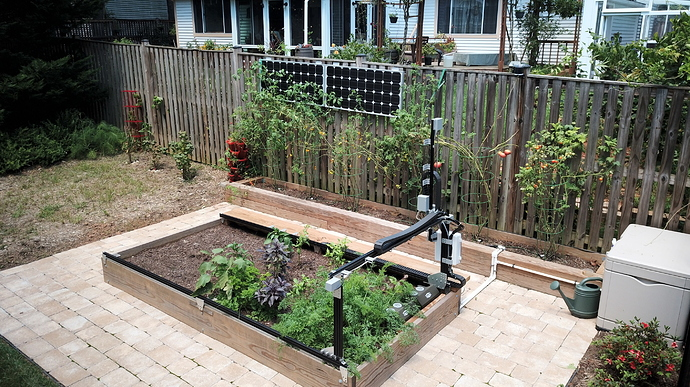
\includegraphics[width=0.75\textwidth]{farmbot.jpeg}
        \end{figure}

        \column{.4\linewidth}
        \begin{figure}
            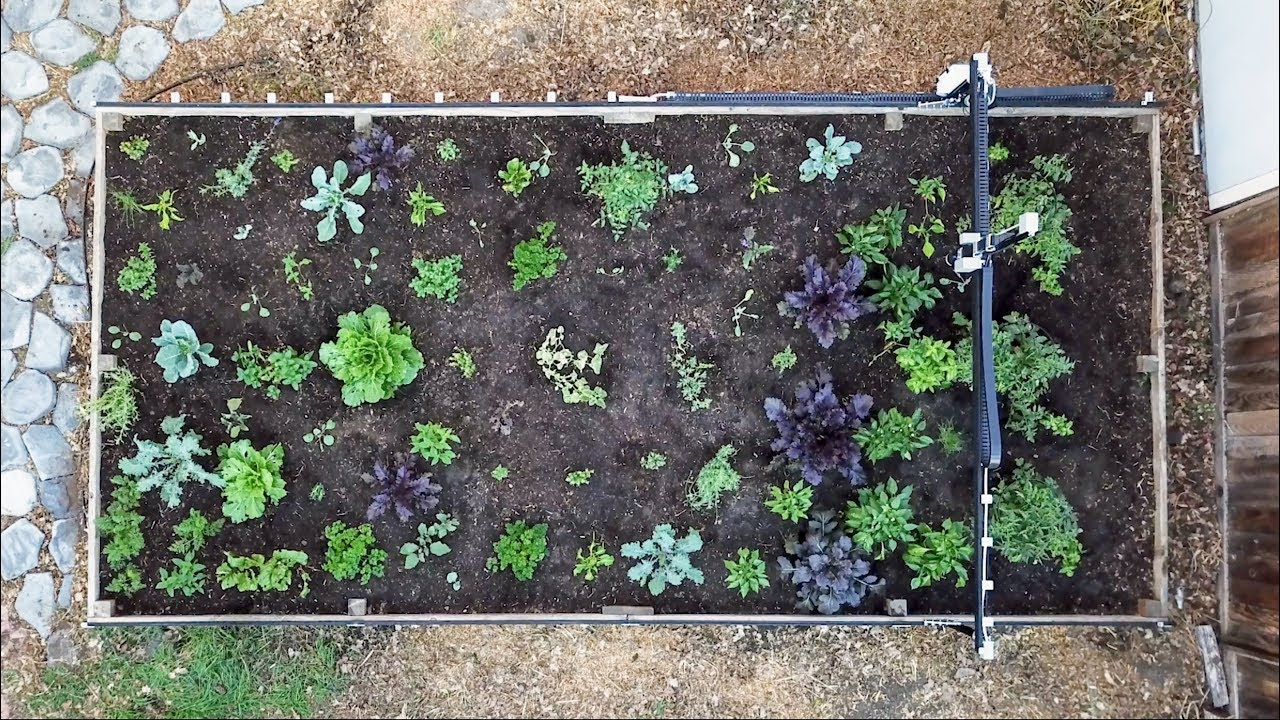
\includegraphics[width=0.75\textwidth]{farmbot-air.jpg}
        \end{figure}
    \end{columns}
\end{frame}

\begin{frame}[t]{Metodologia do Projeto}
    \begin{figure}
        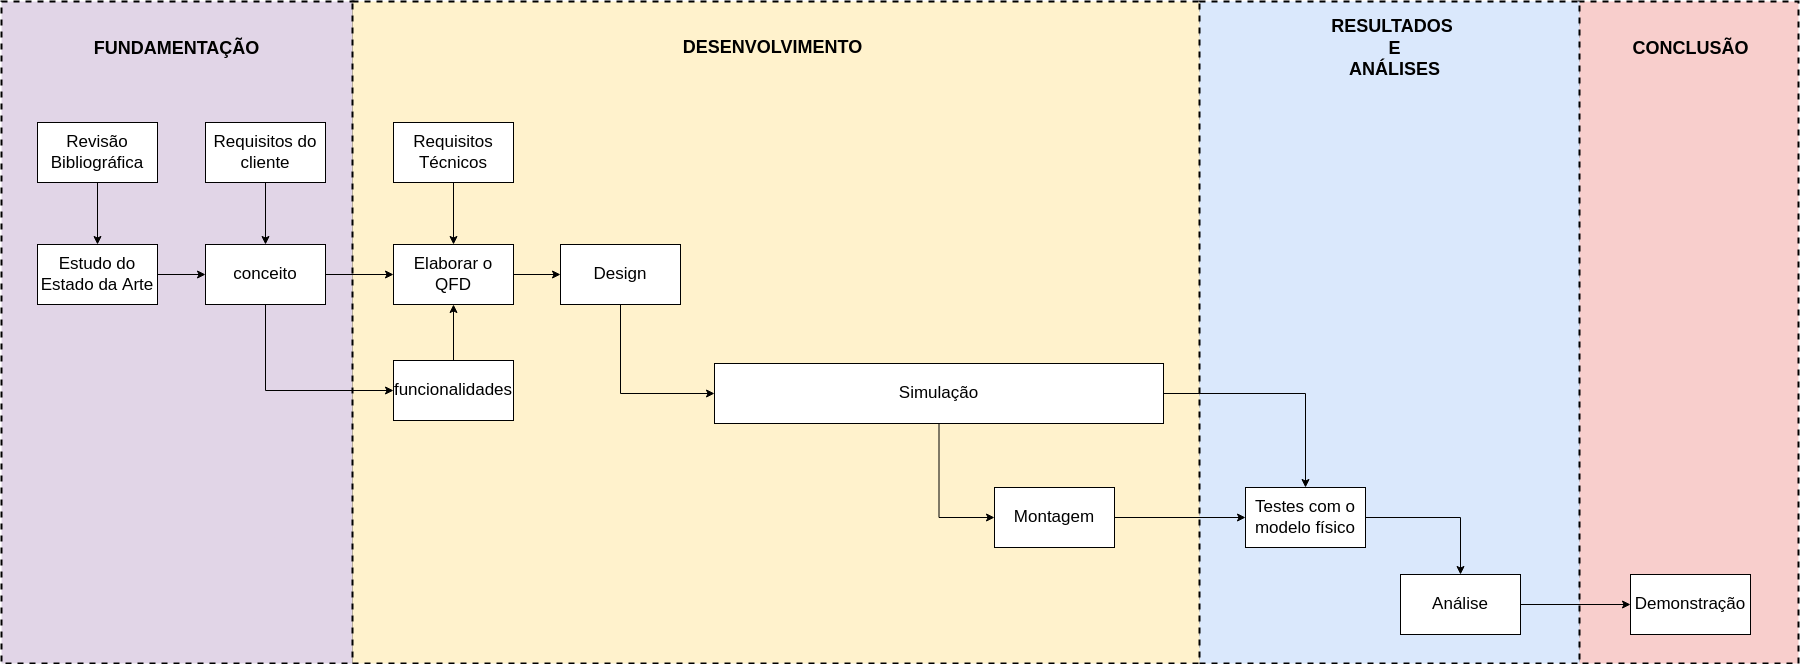
\includegraphics[width=1.005\textwidth]{metodologia.png}
    \end{figure}
\end{frame}

\begin{frame}[t]{O Que Já Foi Desenvolvido}
    \newcommand\vertspacedesenv{0.35cm}

    \begin{columns}[t]
        \column{.05\linewidth}
        \column{.4\linewidth}
            Cronograma do projeto.
            \vspace*{\vertspacedesenv}
        
            Método BILI.
            \vspace*{\vertspacedesenv}
        
            Estudos: C++, Python, R, ROS e modelagem 3D.
            \vspace*{\vertspacedesenv}

            10\% realizado para 9\% planejado.
            \vspace*{\vertspacedesenv}

            29\% planejado até o final do ano.
            \vspace*{\vertspacedesenv}
        \column{.6\linewidth}
        %\centerline{
            \begin{figure}[H]
                \vspace{-0.9cm}
                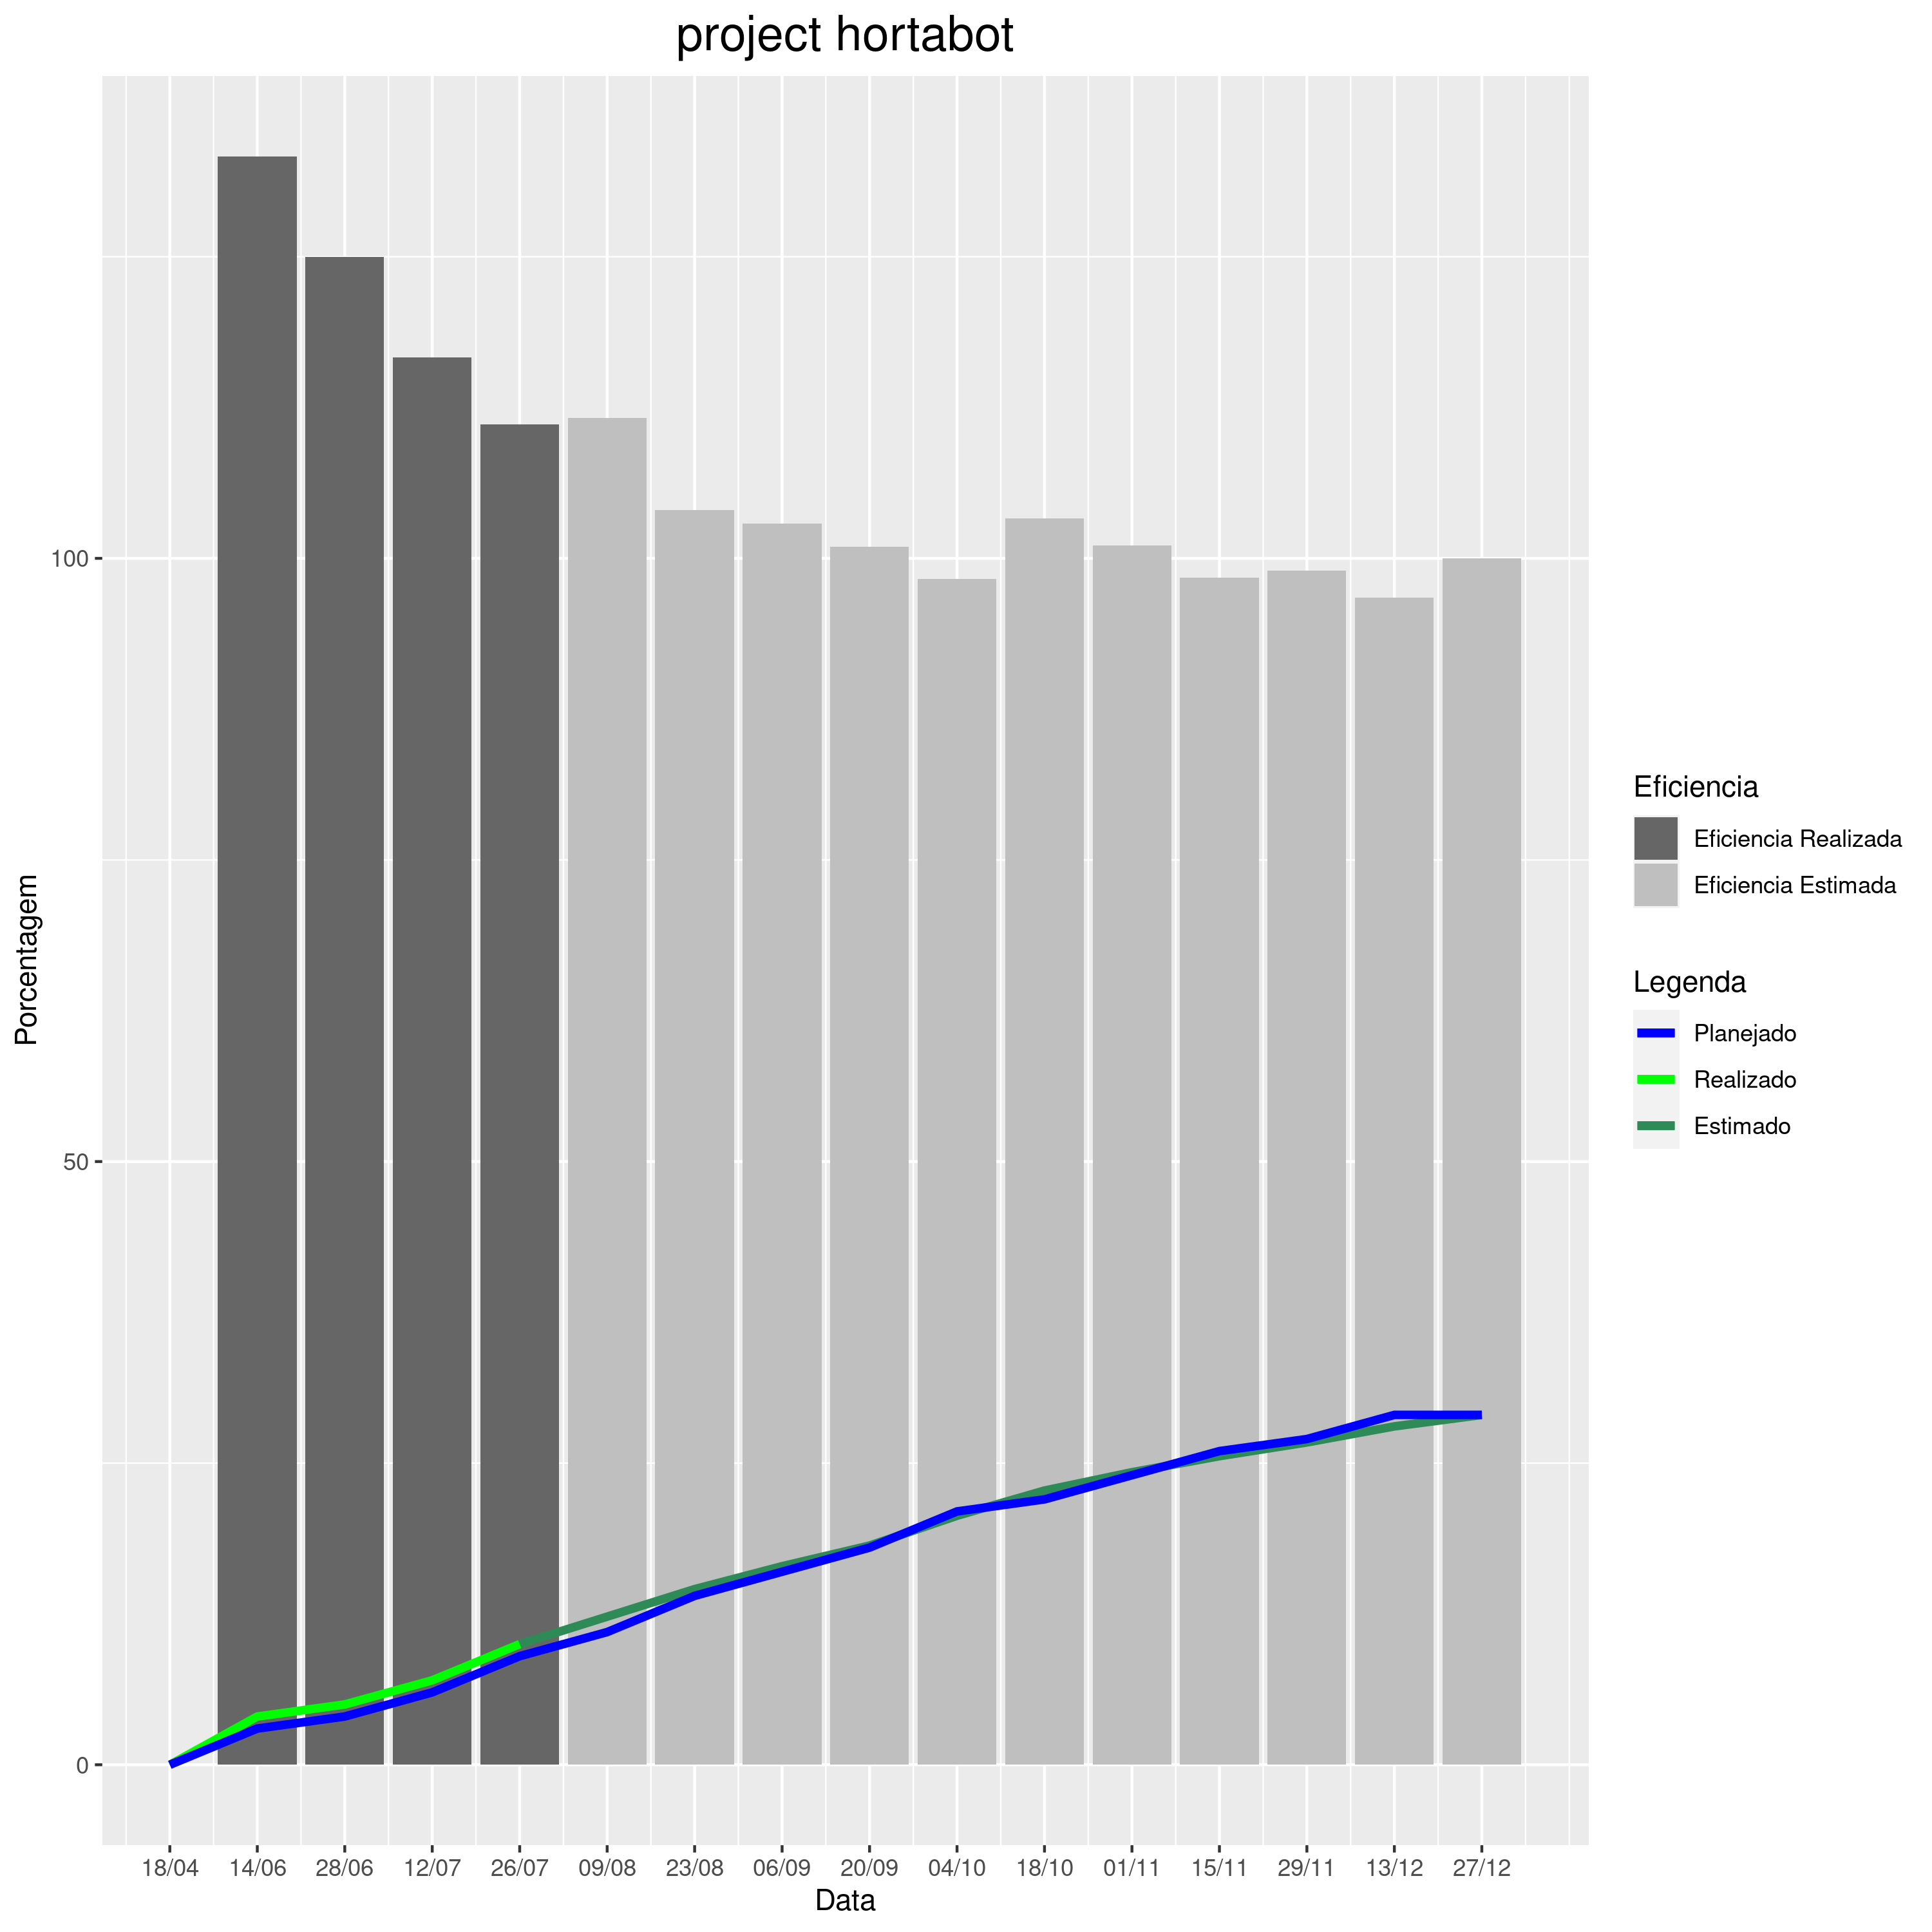
\includegraphics[width=0.78\textwidth]{graph-26-07.png}
            \end{figure}
    \end{columns}

    
\end{frame}

% \begin{frame}[t]{}
%     \begin{figure}
%         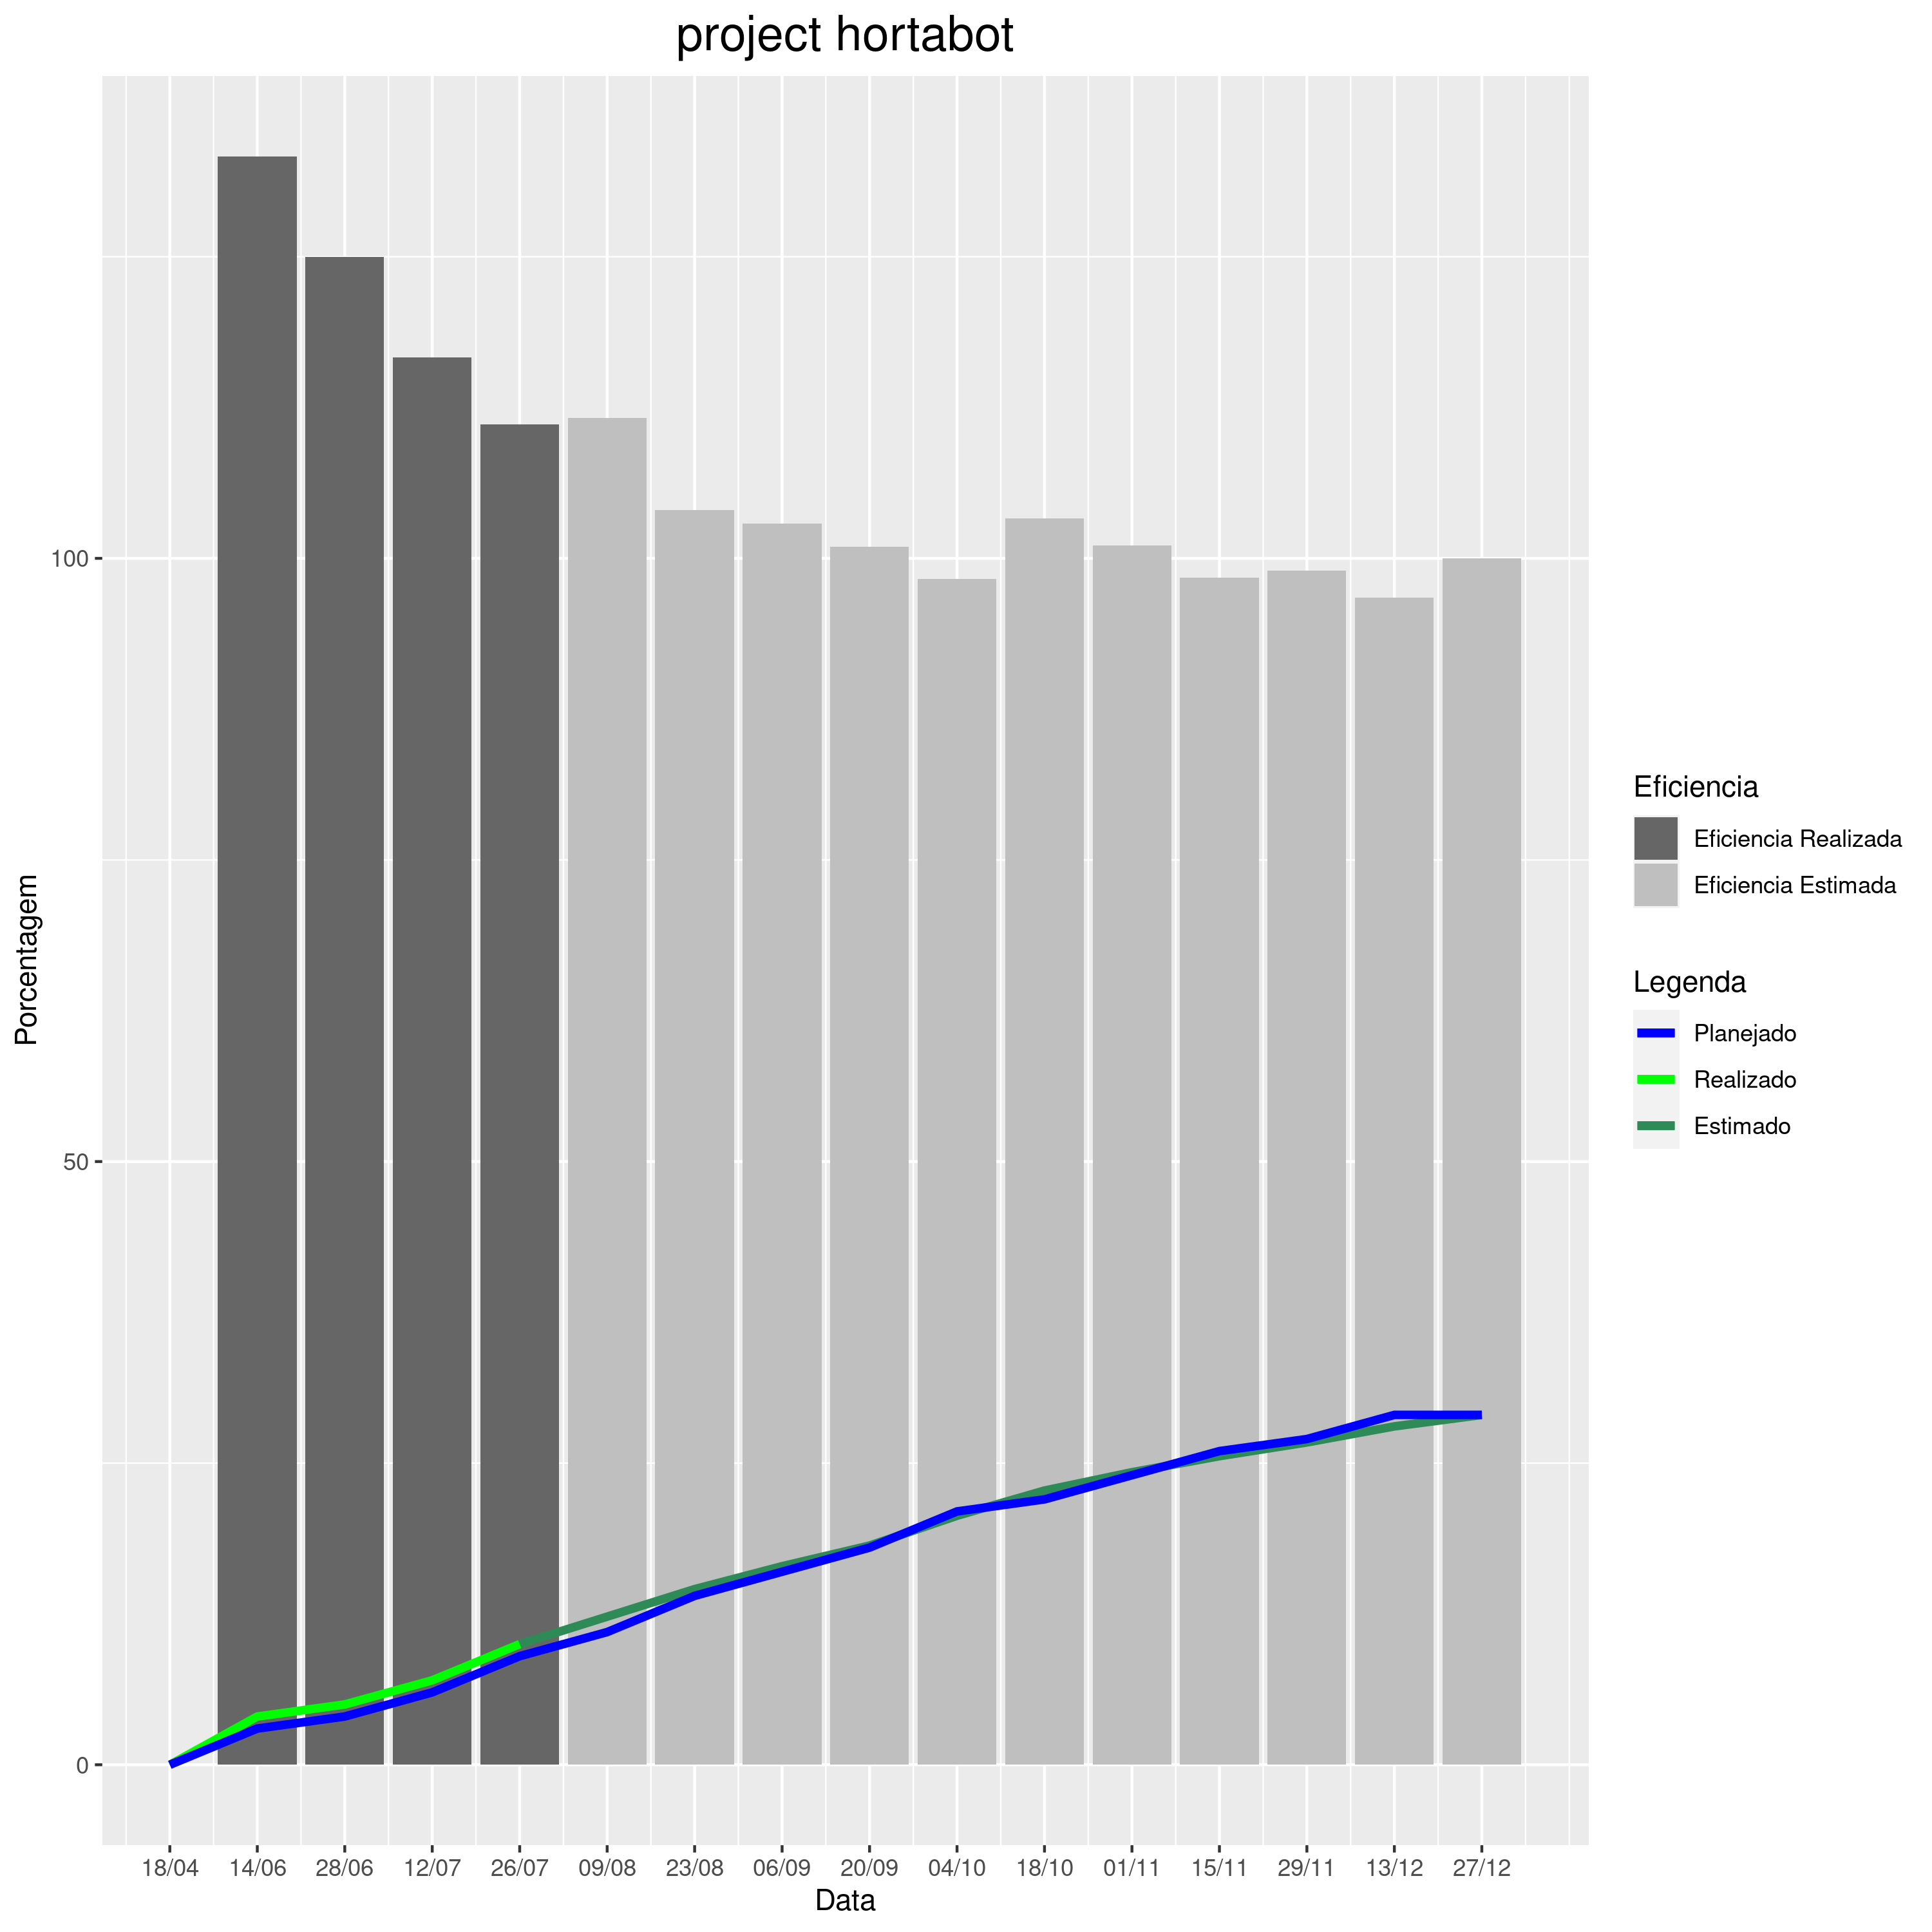
\includegraphics[width=0.58\textwidth]{graph-26-07.png}
%     \end{figure}
% \end{frame}

% \begin{frame}[t]{Artigos Selecionados}
%     \newcommand\vertspaceartigos{0.35cm}

%     Autonomous Agricultural Robot and Its Row Guidance \cite{xue2010autonomous}
%     \vspace*{\vertspaceartigos}

%     Autonomous agricultural robot - conception of inertial navigation system \cite{jasinski2016autonomous}
%     \vspace*{\vertspaceartigos}

%     Sensor and Vision based Autonomous AGRIBOT for Sowing Seeds \cite{santhi2017sensor}
%     \vspace*{\vertspaceartigos}

%     Autonomous agricultural robot - Testing of the vision system for plants/weed classification \cite{jasinski2018autonomous}
%     \vspace*{\vertspaceartigos}

%     GPS Guided Autonomous Navigation of a Small Agricultural Robot with Automated Fertilizing System \cite{khan2018gps}
%     \vspace*{\vertspaceartigos}
% \end{frame}


\begin{frame}[t]{Próximos Passos}
    \newcommand\vertspaceproximos{0.35cm}
    Construir mapa conceitual dos artigos lidos.
    \vspace*{\vertspaceproximos}

    Listar os requisitos técnicos e funcionalidades para desenvolver o design.
    \vspace*{\vertspaceproximos}

    Construir o modelo em ambiente simulado.
    \vspace*{\vertspaceproximos}

    Realizar a montagem e testes com o modelo físico.
    \vspace*{\vertspaceproximos}

    Escrever \textbf{3 artigos} sobre: SOTA (2022.2), Design elaborado (2023.1) e resultados obtidos (2023.2).
    \vspace*{\vertspaceproximos}
\end{frame}
